%!TEX root = ./main.tex

\section[Model]{One Mental Model}

% SECTION TIMING: 22:00--30:00 (3 frames).

% Teaching note (45 s): pause before revealing the four-part model.
\begin{frame}{You press Call. What happens next?}
  \begin{columns}[T,onlytextwidth]
    \column{0.40\textwidth}
      \centering
      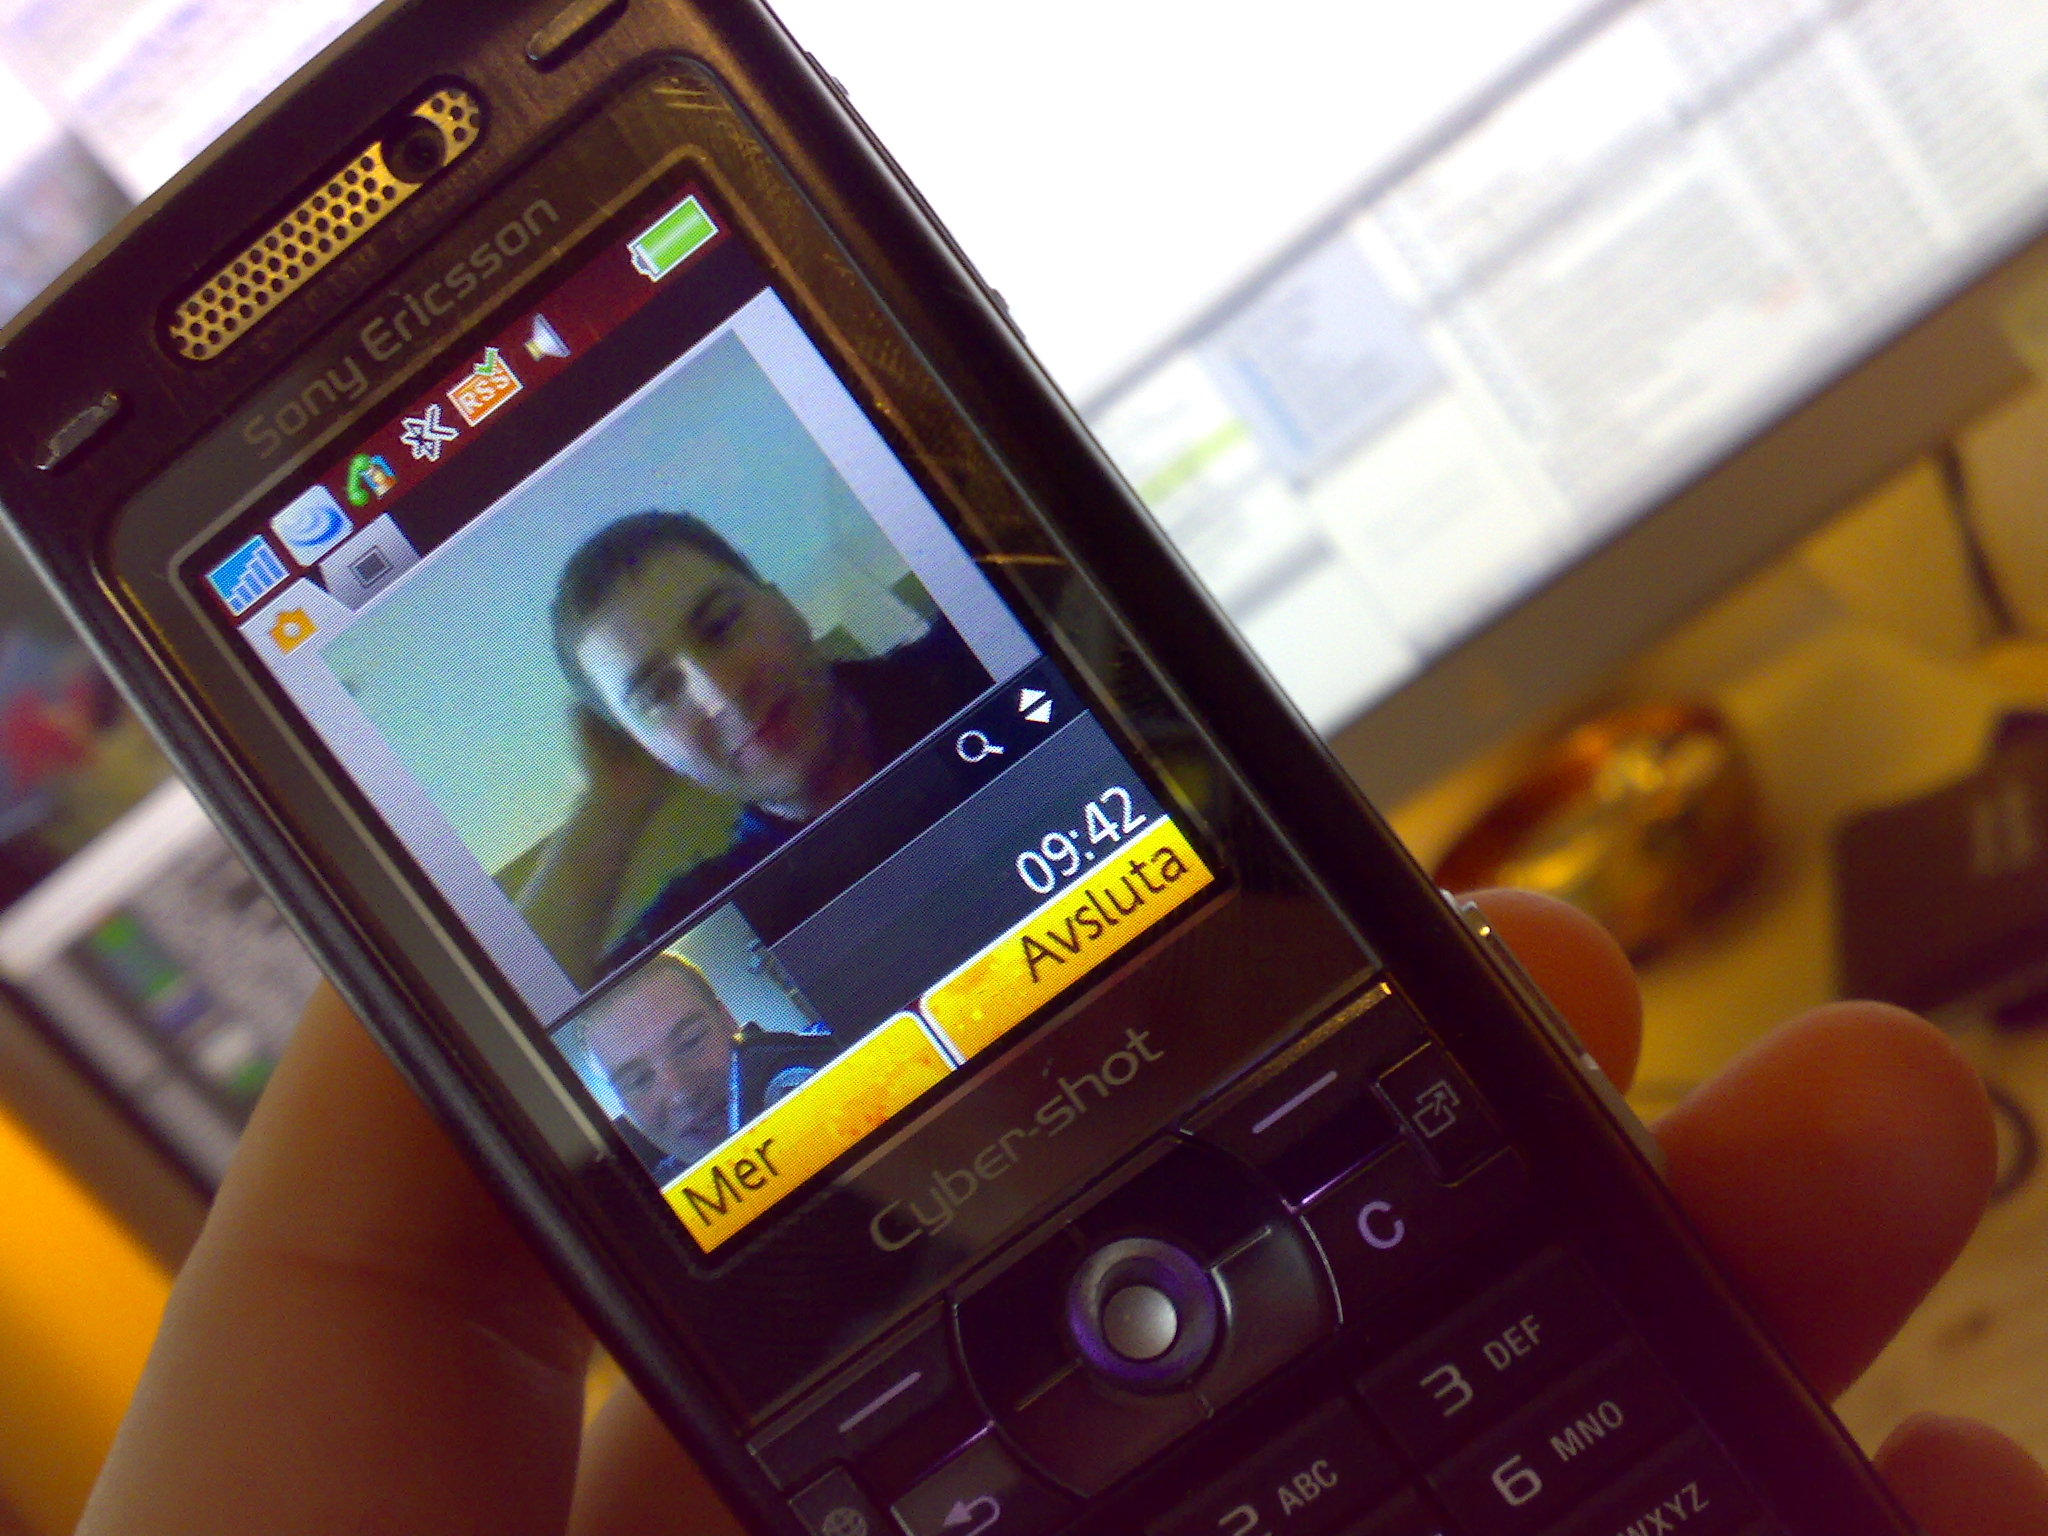
\includegraphics[width=\linewidth]{figure/xg/3g_video_call.jpg}
      \source{https://commons.wikimedia.org/wiki/File:Video_Call.jpg}{UMTS video call}
    \column{0.56\textwidth}
      \large
      Your phone has to find a tower.

      \vspace{0.6em}
      The network has to recognize you.

      \vspace{0.6em}
      Then it has to find the other end.
  \end{columns}

  \vspace{0.4em}
  \qa{Which part of the network handles each of those three jobs?}
     {The RAN finds the tower and holds the radio link. The core recognizes you
      and decides what you may do. The core also reaches the other end, through
      the Internet or the telephone network.}
\end{frame}

\begin{frame}{Four worlds are hiding behind one tap}
  \centering
  \begin{tikzpicture}[node distance=0.30cm]
    \node[netnode,minimum width=2.0cm,font=\small\bfseries] (ue) {UE\\your device};
    \node[netnode,minimum width=2.2cm,font=\small\bfseries,right=of ue] (ran) {RAN\\radio access};
    \node[corenode,minimum width=2.3cm,font=\small\bfseries,right=of ran] (core) {Core\\control + routing};
    \node[netnode,minimum width=2.6cm,font=\small\bfseries,right=of core] (dn) {PSTN / Internet\\destination};
    \draw[flow] (ue) -- (ran);
    \draw[flow] (ran) -- (core);
    \draw[flow] (core) -- (dn);
  \end{tikzpicture}

  \vspace{1.2em}
  \begin{columns}[T,onlytextwidth]
    \column{0.45\textwidth}
      \Large\textcolor{ranblue}{\textbf{RAN}}

      \normalsize Turns radio waves\\into managed links.
    \column{0.51\textwidth}
      \Large\textcolor{coreorange}{\textbf{Core}}

      \normalsize Remembers who you are,\\where you are,\\and what you may do.
  \end{columns}
  \glossline{UE = User Equipment (your phone) \quad RAN = Radio Access Network\\
    PSTN = Public Switched Telephone Network, the traditional telephone network\\
    3GPP = 3rd Generation Partnership Project, the body that writes these standards}
  \source{https://www.3gpp.org/technologies/5g-system-overview}{Conceptual model based on 3GPP system architecture}
\end{frame}

\begin{frame}{The network still has the same six jobs}
  \vspace{0.5em}
  \begin{columns}[T,onlytextwidth]
    \column{0.46\textwidth}
      \large
      \begin{enumerate}\itemsep5pt
        \item Find a cell
        \item Request access
        \item Prove identity
      \end{enumerate}
    \column{0.50\textwidth}
      \large
      \begin{enumerate}\itemsep5pt
        \setcounter{enumi}{3}
        \item Get radio resources
        \item Route voice or data
        \item Move without dropping
      \end{enumerate}
  \end{columns}

  \vspace{1.0em}
  \takeaway{The node names change.\\The jobs are surprisingly persistent.}
\end{frame}
